\documentclass{article}
\usepackage{graphicx} % Required for inserting images
\usepackage[T2A]{fontenc}   % Кодировка шрифтов для кириллицы
\usepackage[utf8]{inputenc} % Кодировка входного файла (UTF-8)
\usepackage[english,russian]{babel} % Языковая поддержка
\usepackage{hyperref}
\title{Мини-конспект по теме: Теорема Пифагора}
\author{Автор: Я Сам}
\date{16 июля 2025 г.}

\begin{document}
\maketitle
\tableofcontents{}
\newpage
\section{Введение}
Теорема Пифагора — одна из важнейших теорем евклидовой геометрии. Она находит применение в самых разных областях:
\begin {itemize}
    \item  геометрия и тригонометрия
    \item физика
    \item инженерные расчеты
    \item компьютернаяграфика
\end {itemize}



\section{Формулировка теоремы}
\textbf{Слова: }  В прямоугольном треугольнике квадрат гипотенузы равен сумме квадратов катетов.
\begin {equation}
    c^2 = a^2 + b^2
\end{equation}
Как видно из формулы 1, знание двух сторон позволяет найти третью.



\section{ Доказательство (набросок)}
Одно из доказательств основывается на площади квадрата, составленного
из четырёх одинаковых прямоугольных треугольников и малого квадрата
в центре. Раскладывая площадь двумя способами, получаем $c^2 = a^2 +b^2$.


\section{Примеры расчёта}
\paragraph{Пример 1}
\begin{center}
    a = 3, b = 4
\end{center}
\[
    c = \sqrt{a^2 + b^2} = \sqrt{9 + 16} = 5
\]

\paragraph{Пример 2}
\begin{enumerate}
    \item Дано: a = 5, b = 12
    \item Решение:
    \[
        c = \sqrt{5^2 + 12^2} = \sqrt{25 + 144} = 13
    \]
\end{enumerate}


\section{Таблица значений}
\begin{center}
\begin {tabular} {|c|c|c|}
    \hline
        Катет a & Катет b & Гипотенуза с \\
    \hline
        3 & 4 & 5 \\
    \hline
        5 & 12 & 13 \\
    \hline
        7 & 24 & 25 \\
        \hline
\end{tabular}
\end{center}


\section{Иллюстрация}
Ниже пример изображения (не забудьте добавить файл triangle.png в ту же папку):

\begin{center}
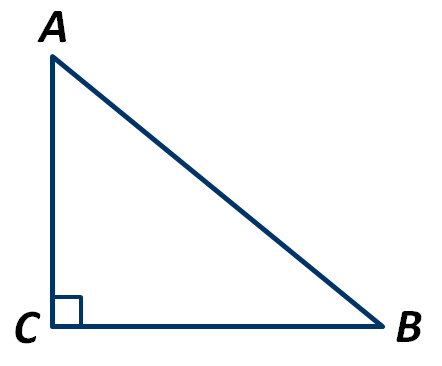
\includegraphics [width = 0.5 \textwidth]
{triangle.png}
\end{center}



\section{Заключение}
Теорема Пифагора — один из краеугольных камней геометрии, помогающий решать
множество практических задач.



\section{Ссылки и литература}
\begin{itemize}
    \item Википедия: \href {https://ru.wikipedia.org/wiki/%D0%A2%D0%B5%D0%BE%D1%80%D0%B5%D0%BC%D0%B0_%D0%9F%D0%B8%D1%84%D0%B0%D0%B3%D0%BE%D1%80%D0%B0} {Теорема Пифагора}
    \item Классические учебники геометрии


\end{document}